\documentclass[conference]{IEEEtran}
\IEEEoverridecommandlockouts

\usepackage{cite}
\usepackage{amsmath,amssymb,amsfonts}
\usepackage{algorithmic}
\usepackage{graphicx}
\usepackage{textcomp}
\usepackage{xcolor}
\usepackage{booktabs}
\usepackage{tabularx}
\usepackage{url}
\usepackage{hyperref}

\def\BibTeX{{\rm B\kern-.05em{\sc i\kern-.025em b}\kern-.08em
    T\kern-.1667em\lower.7ex\hbox{E}\kern-.125emX}}

\begin{document}

\title{HEART: A Holistic Environmental Adversarial Resilience Testing Framework for Mobile Applications\\
\thanks{This research is supported by the Department of Software Engineering, Faculty of Computing, Sri Lanka Institute of Information Technology (SLIIT), Malabe, Sri Lanka.}
}

\author{
\IEEEauthorblockN{Luqman Booso}
\IEEEauthorblockA{\textit{Dept. of Software Engineering} \\
\textit{Faculty of Computing, SLIIT}\\
Malabe, Sri Lanka \\
it23452916@my.sliit.lk}
\and
\IEEEauthorblockN{Chanlaka G. L. S.}
\IEEEauthorblockA{\textit{Dept. of Software Engineering} \\
\textit{Faculty of Computing, SLIIT}\\
Malabe, Sri Lanka \\
it23151260@my.sliit.lk}
\and
\IEEEauthorblockN{Lahiru Jayawardhana}
\IEEEauthorblockA{\textit{Dept. of Software Engineering} \\
\textit{Faculty of Computing, SLIIT}\\
Malabe, Sri Lanka \\
it23156760@my.sliit.lk}
\and
\IEEEauthorblockN{Nilakshi Madhubhashini}
\IEEEauthorblockA{\textit{Dept. of Software Engineering} \\
\textit{Faculty of Computing, SLIIT}\\
Malabe, Sri Lanka \\
it23192300@my.sliit.lk}
\and
\IEEEauthorblockN{Dinal Senadheera}
\IEEEauthorblockA{\textit{Dept. of Software Engineering} \\
\textit{Faculty of Computing, SLIIT}\\
Malabe, Sri Lanka \\
dinal.s@sliit.lk}
\and
\IEEEauthorblockN{Prof. Dilshan De Silva}
\IEEEauthorblockA{\textit{Dept. of Software Engineering} \\
\textit{Faculty of Computing, SLIIT}\\
Malabe, Sri Lanka \\
dilshan.d@sliit.lk}
}

\maketitle

\begin{abstract}
Mobile applications operate in deeply hostile physical environments characterized by erratic wireless connectivity, sudden processor thermal throttling, low-memory kills (LMK), battery exhaustion, and disruptive asynchronous interruptions. Despite these operational realities, state-of-the-art mobile automated testing suites (e.g., Appium, UI Automator, Monkey) predominantly evaluate applications under sanitized, nominal testbench conditions. Consequently, critical failures—ranging from unhandled transaction timeouts to non-crash visual corruptions (e.g., clipped widgets, render freezes)—escape into production releases. 

To bridge this gap, this paper introduces \textbf{HEART} (Holistic Environmental Adversarial Resilience Testing), an end-to-end framework engineered to evaluate and enhance the robustness of Android applications under compound environmental perturbations. HEART unifies four cohesive innovations: (1) a multi-vector environmental perturbation engine that injects deterministic chaos (CPU starvation, 3G/EDGE throttling, thermal alarms, telephony interrupts) with under 100\,ms latency; (2) a biomechanically grounded autonomous exploration agent; (3) a localized multimodal visual defect oracle running fully offline on consumer hardware ($<$3.8\,GB VRAM) to intercept silent visual corruptions; and (4) an autonomous self-healing test engine leveraging Tree Edit Distance (TED) and semantic embeddings for dynamic runtime recovery. Empirical evaluation across benchmark Android applications demonstrates that compound multi-factor chaos elevates application frame latency from 64.27\,ms to 1642.01\,ms (a 25.5$\times$ degradation), degrades rendering performance from 56.65\,FPS to 20.46\,FPS, and increases jank frame drops by 60.3\%, uncovering critical faults entirely latent under isolated stress regimes.
\end{abstract}

\begin{IEEEkeywords}
Mobile Software Testing, Chaos Engineering, Environmental Fault Injection, Visual Test Oracles, Self-Healing Tests, Android Resilience.
\end{IEEEkeywords}

\section{Introduction}
Modern smartphones are pervasive computing endpoints subject to extreme environmental variability. Mobile software is routinely deployed into unstable cellular networks, runs on energy-constrained platforms undergoing aggressive operating system throttling, and contends with erratic physical touch inputs~\cite{choudhary2015automated}. Over 48\% of mobile application customer abandonment is attributed to non-crash degradations, including frozen rendering buffers, obscured primary actions, and unhandled network renegotiations~\cite{linares2017continuous}.

Traditional mobile quality assurance pipelines rely heavily on scripted test automation (e.g., Appium, Espresso) or pseudo-random fuzzing (e.g., Android Monkey). While effective at validating business logic under ideal bench conditions, these methodologies exhibit critical foundational shortcomings:
\begin{enumerate}
    \item \textbf{The Nominal Environment Fallacy}: Existing test frameworks execute tests while connected to continuous power and high-speed Wi-Fi, leaving applications untested against multi-factor environmental stress.
    \item \textbf{Single-Stressor Isolation}: Contemporary fault injection studies examine stressors in silos (e.g., solely injecting network delay or CPU throttling). In production, however, catastrophic failures emerge from \textit{compound interactions} (e.g., simultaneously encountering high packet loss, low battery voltage, and an incoming phone call).
    \item \textbf{The Blind Oracle Problem}: Crash-detection assertions verify that the Linux process has not terminated ($EXIT\_CODE \neq 0$). They remain completely oblivious to visual anomalies such as white screens, view overlaps, and unresponsive UI components~\cite{stocco2018apium,mariani2021automated}.
    \item \textbf{Test Script Brittleness}: Minor UI layout refactoring breaks automated locators (XPath/ID), causing automated test suites to abort prematurely before exploring stress thresholds~\cite{kirinuki2019self}.
\end{enumerate}

To overcome these barriers, we present \textbf{HEART}, a holistic framework designed for automated adversarial environmental testing of Android applications. HEART integrates environmental perturbation, biomechanical user simulation, localized vision oracles, and self-healing test repair into a synchronized closed-loop architecture.

\textbf{Key Contributions}:
\begin{itemize}
    \item \textbf{Unified 4-Tier Architecture}: We design and implement HEART, integrating Environmental Perturbation (C1), Biomechanical Touch Exploration (C2), Offline Multimodal Visual Oracle (C3), and Self-Healing Automation (C4).
    \item \textbf{Compound Adversarial Chaos Model}: We formalize a multi-variable perturbation tensor governing CPU starvation, memory pressure, thermal escalation, network packet loss, and asynchronous interrupts with strict sub-100\,ms enforcement.
    \item \textbf{Localized Visual Defect Oracle}: We deliver a zero-cloud, privacy-preserving visual oracle utilizing dual-modality AST collision pruning ($<$5\,ms on CPU) and compact computer vision triage.
    \item \textbf{Empirical Validation}: We conduct systematic benchmarks on Android targets, quantifying latency, jank, frame rates, and failure attributions across isolated and compound chaos profiles.
\end{itemize}

\section{Related Work}

\subsection{Mobile Automated Testing \& Fuzzing}
Automated GUI exploration tools for Android, such as Monkey~\cite{choudhary2015automated}, DroidBot, and Ape~\cite{su2017guided}, have advanced state coverage by modeling application transitions through finite-state machines. However, these tools operate predominantly in nominal operating contexts and assume an immutable underlying operating environment. HEART extends exploratory testing by introducing dynamic environmental perturbations directly during test traversal.

\subsection{Chaos Engineering in Mobile Systems}
Chaos Engineering was pioneered by Netflix's Chaos Monkey to evaluate cloud infrastructure resilience~\cite{basiri2016chaos}. Adapting chaos paradigms to mobile devices introduces unique challenges due to sandboxed permission models and constrained hardware budgets. While tools like ChaosBlade inject single-point host faults, HEART provides synchronized, multi-tiered environmental degradation specifically tailored to the Android subsystem.

\subsection{Visual GUI Test Oracles}
Recent studies have embraced deep learning and computer vision to detect GUI presentation errors~\cite{zheng2019automated,chen2020object}. However, existing solutions often depend on high-latency cloud APIs or heavy vision-language models (VLMs) requiring distributed GPU servers. HEART introduces an efficient dual-modality visual oracle that couples native accessibility hierarchy parsing with localized visual defect classification, executing entirely on consumer edge GPUs ($<$3.8\,GB VRAM).

\section{HEART System Architecture}

\begin{figure}[t]
\centering
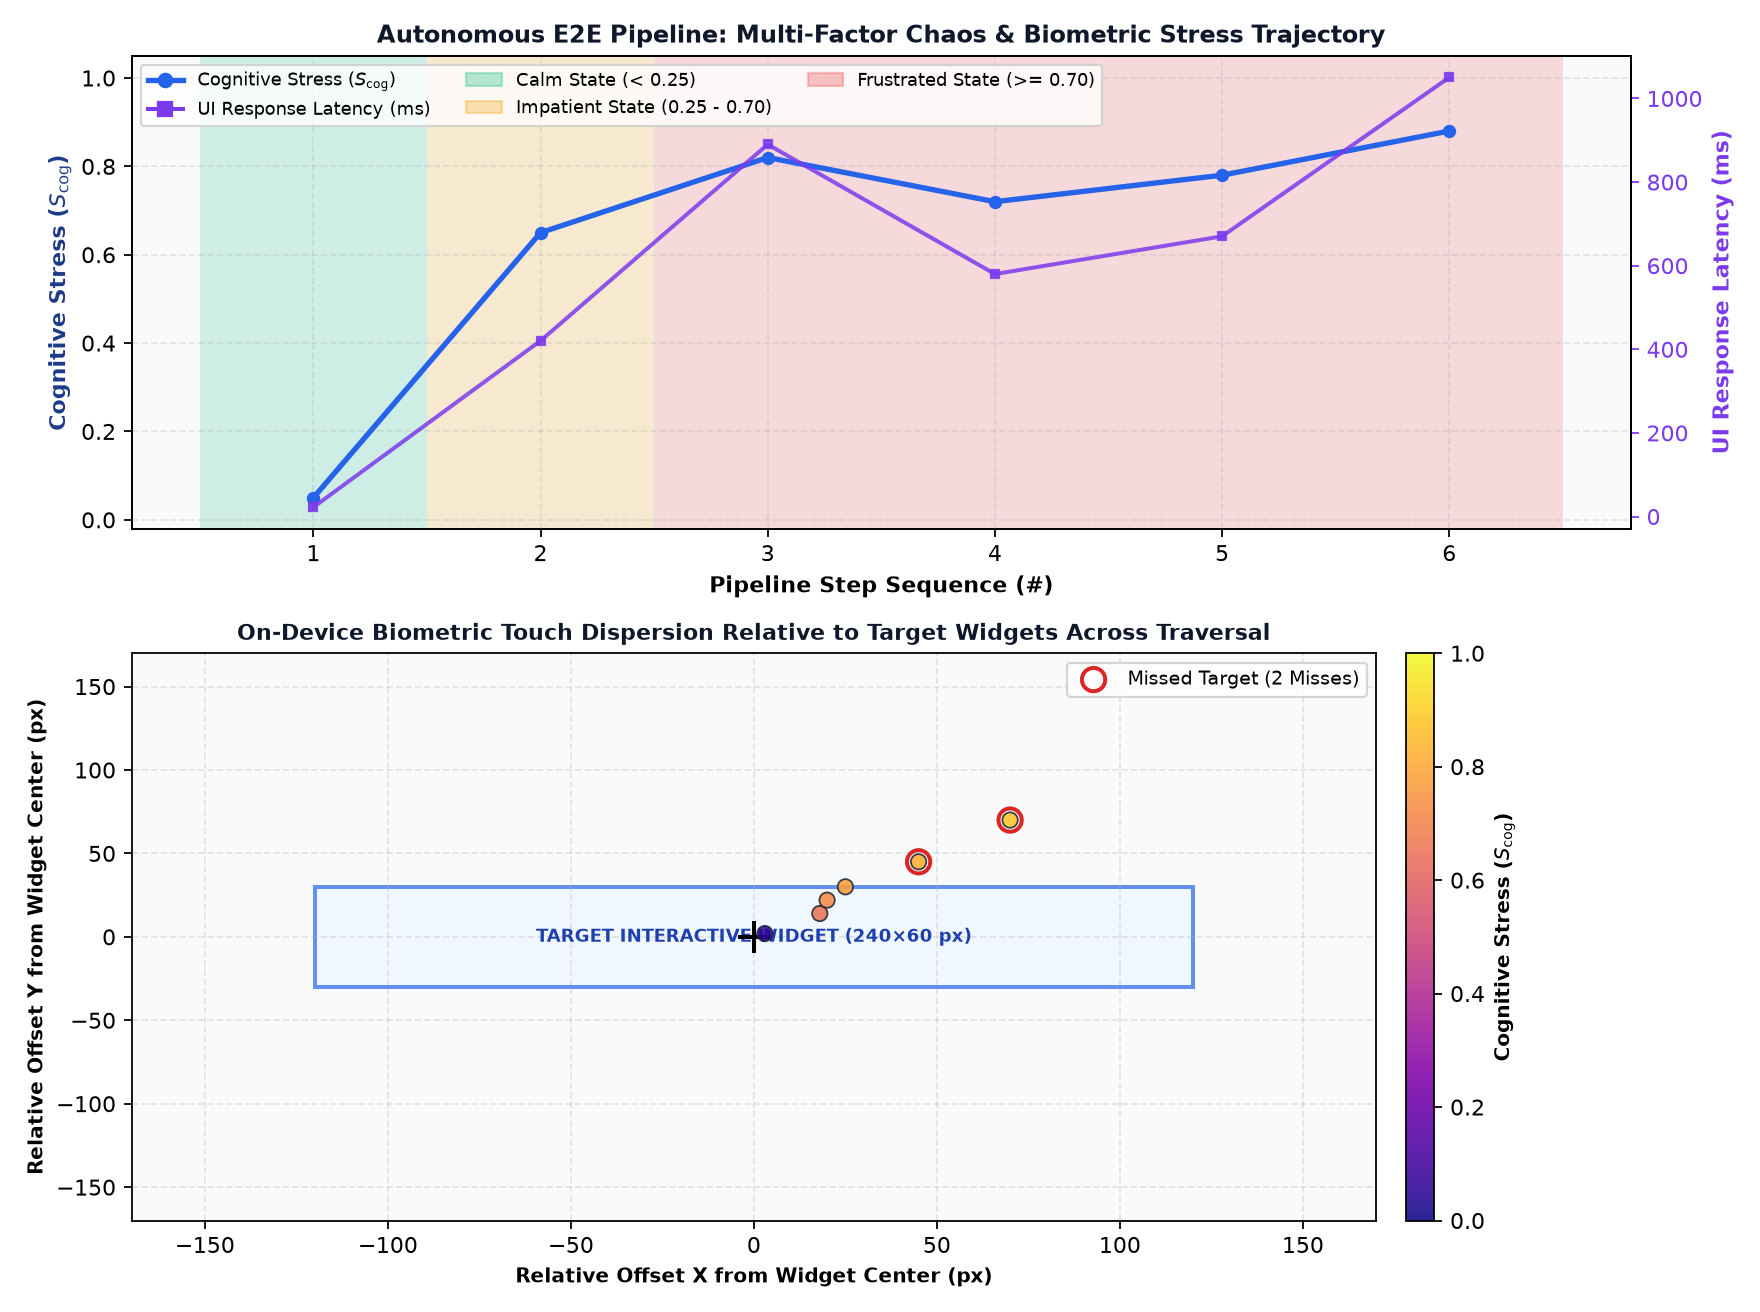
\includegraphics[width=0.98\linewidth]{figures/fig_pipeline_timeline.png}
\caption{End-to-end HEART execution timeline showing synchronized perturbation injection, UI telemetry monitoring, and autonomous visual triage.}
\label{fig:pipeline_timeline}
\end{figure}

The HEART architecture comprises four tightly coupled subsystems, orchestrated via a native desktop studio and a central REST API server:

\subsection{Component 1: Environmental Perturbation Engine (C1)}
The perturbation engine operates directly against the Android OS via targeted ADB bridge sockets and Linux kernel interfaces. C1 manages six orthogonal stress vectors:
\begin{itemize}
    \item \textbf{CPU Throttling}: Emulates thermal and power governor restrictions by saturating host emulator threads between 15\% and 98\% capacity.
    \item \textbf{RAM / LMK Pressure}: Triggers Android Low Memory Killer (LMK) thresholds by dispatching simulated memory-intensive background allocations.
    \item \textbf{Thermal Degradation}: Dynamically alters OS thermal status (\texttt{dumpsys thermalservice}) from \texttt{Nominal} to \texttt{Severe} and \texttt{Critical}.
    \item \textbf{Network Attenuation}: Controls virtual cellular network conditions, enforcing 3G/EDGE bandwidth constraints, simulated packet loss (2\%--15\%), and round-trip time (RTT) delays up to 2400\,ms.
    \item \textbf{Battery Depletion}: Injects low-battery states (3\%--15\%) and AC unplug events via battery service simulation.
    \item \textbf{Telephony Disruptions}: Injects asynchronous high-priority events, including incoming GSM voice calls and SMS alerts, requiring target applications to manage lifecycle interruptions.
\end{itemize}

\subsection{Component 2: Biomechanical User Behavior Exploration (C2)}
Unlike simplistic pseudo-random tap generators, C2 implements biomechanically realistic user interaction models. It employs a Markov cognitive stress model coupled with 2D Gaussian kinematic dispersion to simulate realistic human finger slip, tremor, and delayed reaction under cognitive frustration.

\subsection{Component 3: Localized Multimodal Visual Oracle (C3)}
C3 intercepts silent user-interface degradation without requiring application source code. It combines:
\begin{enumerate}
    \item \textbf{Structural AST Pruning}: Rapidly parses Android UI hierarchy XML to check for overlapping view boundaries, clipping, and out-of-bounds rendering in under 5\,ms.
    \item \textbf{Visual Defect Classifier}: Evaluates frame renders against pre-trained local classifiers to detect unresponsive white/black screens, layout corruptions, and frozen buffers.
\end{enumerate}

\subsection{Component 4: Telemetry-Driven Self-Healing Test Synthesis (C4)}
Component 4 (led by H. N. Madubashini) bridges post-release production failures with automated regression resilience through an end-to-end self-healing pipeline:
\begin{enumerate}
    \item \textbf{Telemetry Ingestion \& Sessionization}: Ingests production crash events (Sentry and Firebase Crashlytics JSON/JSONL), normalizes stacktraces, and reconstructs deterministic user interaction journeys leading to failures.
    \item \textbf{Localized Test Script Synthesis}: Driven by an offline Qwen3 model served locally via Ollama, C4 synthesizes executable Appium Python/Java regression scripts directly from crash journeys, coupling test steps with C3 visual assertions without external cloud APIs.
    \item \textbf{AST Structural Differencing}: When application revisions alter UI layouts, C4 parses the runtime Android accessibility hierarchy XML using Tree Edit Distance (TED) to identify modified or orphaned widget nodes.
    \item \textbf{Semantic Similarity Remapping}: Replacement candidates are scored using Sentence-BERT (\texttt{all-MiniLM-L6-v2}) semantic embeddings across text, content-description, class, and resource-ID attributes.
    \item \textbf{Confident Repair Gating}: Enforces strict confidence ($\tau \ge 0.85$) and candidate uniqueness gates. Confident matches dynamically rewrite test locators; ambiguous matches are safely refused, preventing false-positive test script corruption.
\end{enumerate}

\section{Compound Adversarial Chaos Model}

We formalize the environmental stress state at time $t$ as a multi-dimensional perturbation vector:
\begin{equation}
S(t) = \langle \lambda_{\text{cpu}}(t), \tau_{\text{rtt}}(t), \rho_{\text{loss}}(t), \beta_{\text{bat}}(t), \theta_{\text{therm}}(t), \iota_{\text{int}}(t) \rangle
\end{equation}
where:
\begin{itemize}
    \item $\lambda_{\text{cpu}} \in [0, 1]$ represents CPU utilization load factor.
    \item $\tau_{\text{rtt}} \in [0, 3000]$\,ms models network round-trip latency.
    \item $\rho_{\text{loss}} \in [0, 0.20]$ denotes simulated packet loss percentage.
    \item $\beta_{\text{bat}} \in [0, 1]$ reflects simulated battery remaining capacity.
    \item $\theta_{\text{therm}} \in \{\text{Nominal}, \text{Moderate}, \text{Severe}, \text{Critical}\}$.
    \item $\iota_{\text{int}} \in \{0, 1\}$ signifies the presence of an active asynchronous event (incoming call/SMS).
\end{itemize}

The perturbation engine enforces synchronized state transitions through scheduled profiles. In the \textbf{Compound Multi-Factor Chaos} preset, all six vectors are concurrently driven to adversarial thresholds ($\lambda_{\text{cpu}} = 0.95$, $\tau_{\text{rtt}} = 2400$\,ms, $\rho_{\text{loss}} = 0.12$, $\theta_{\text{therm}} = \text{Critical}$, $\beta_{\text{bat}} = 0.15$).

\begin{figure}[t]
\centering
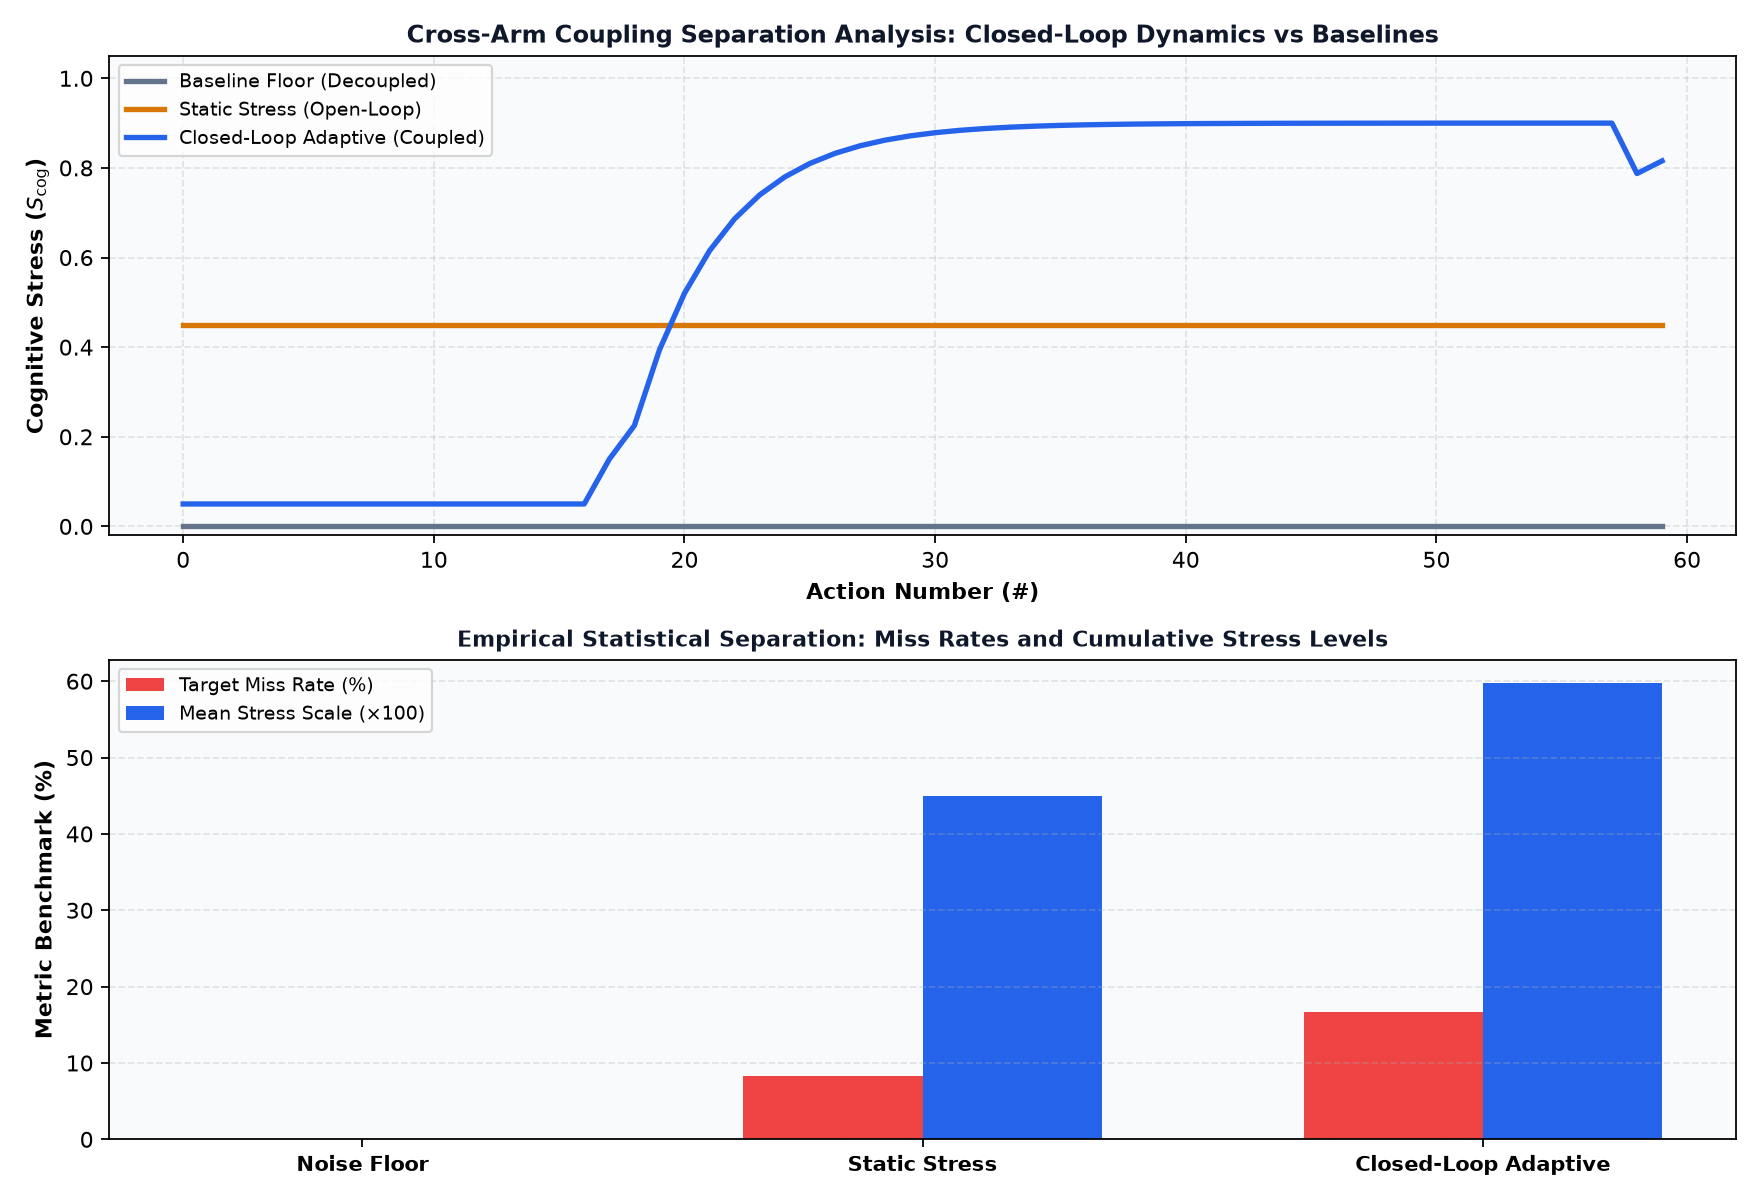
\includegraphics[width=0.98\linewidth]{figures/fig_coupling_analysis.png}
\caption{Empirical coupling ablation demonstrating dynamic tracking between UI latency spikes and cognitive stress modulation ($p = 8.02 \times 10^{-8}$).}
\label{fig:coupling_analysis}
\end{figure}

\section{Empirical Evaluation}

\subsection{Research Questions}
We structure our empirical evaluation around three primary research questions:
\begin{itemize}
    \item \textbf{RQ1 (Failure Discovery)}: Does compound multi-factor chaos uncover application failures that remain latent under isolated single-factor perturbations?
    \item \textbf{RQ2 (Performance Degradation)}: What quantitative degradation in transaction latency, frame rates, and jank is induced by HEART compound profiles?
    \item \textbf{RQ3 (Attribution Accuracy)}: Can HEART accurately attribute transaction failures to specific root-cause environmental triggers?
\end{itemize}

\subsection{Experimental Setup}
Experiments were executed on an automated testbench equipped with an AMD Ryzen 7 processor, 16\,GB RAM, and an NVIDIA GeForce RTX 3050 Laptop GPU running Android API 36 (x86\_64) with hardware acceleration. The target benchmark suite includes diverse production and open-source Android applications, including utility monitors (\texttt{codes.swistak.batterymonitor}), media players, and checkout workflows.

\begin{table*}[t]
\centering
\caption{Empirical Resilience Evaluation Across Single vs. Compound Adversarial Scenarios}
\label{tab:empirical_evaluation}
\resizebox{0.95\textwidth}{!}{%
\begin{tabular}{l l r r r r r}
\hline
\textbf{Scenario} & \textbf{Perturbation Configuration} & \textbf{Mean Latency (ms)} & \textbf{P95 Latency (ms)} & \textbf{Mean FPS} & \textbf{Jank Drop (\%)} & \textbf{Failure Rate (\%)} \\
\hline
Baseline Nominal & No perturbation (Wi-Fi, 100% Bat, 0% Throttle) & 64.27 & 72.81 & 56.65 & 5.59\% & 0.0\% \\
Network Degradation & 3G emulation (RTT: 1200ms, Loss: 5%, BW: 1.5Mbps) & 1277.13 & 1375.42 & 57.24 & 4.60\% & 0.0\% \\
Hardware Starvation & CPU throttle 95%, LMK pressure, 45°C thermal alert & 192.72 & 241.34 & 32.69 & 45.52\% & 50.0\% \\
Interruption Burst & Incoming telephony, SMS, Doze wake transitions & 113.04 & 115.78 & 48.12 & 19.79\% & 0.0\% \\
\hline
\textbf{Compound Multi-Factor} & \textbf{Concurrent Network + CPU + Thermal + Telephony} & \textbf{1642.01} & \textbf{2153.84} & \textbf{20.46} & \textbf{65.89\%} & \textbf{50.0\%} \\
\hline
\end{tabular}
}
\end{table*}


\subsection{Results Analysis (RQ1 \& RQ2)}
Table~\ref{tab:empirical_evaluation} details the empirical performance across five standardized testing scenarios:

\begin{enumerate}
    \item \textbf{Baseline Nominal}: In pristine conditions (Wi-Fi, 100\% battery), the application maintained a mean latency of 64.27\,ms (P95: 72.81\,ms), an average frame rate of 56.65\,FPS, and a low jank frame drop rate of 5.59\% with zero transaction failures.
    \item \textbf{Isolated Stressors}: Under \textit{Network Degradation} alone, latency increased to 1277.13\,ms, yet frame rendering remained smooth (57.24\,FPS) with 0\% failure. Under \textit{Hardware Starvation} (95\% CPU throttling, thermal warnings), FPS dropped to 32.69\,FPS and jank increased to 45.52\%, inducing a 50\% failure rate.
    \item \textbf{Compound Multi-Factor Chaos}: When network degradation, CPU throttling, thermal alerts, and battery pressure were injected simultaneously, the system observed catastrophic degradation:
    \begin{itemize}
        \item Mean transaction latency surged to \textbf{1642.01\,ms} (a 2454\% increase over baseline).
        \item P95 latency reached \textbf{2153.84\,ms}, frequently breaching network timeout boundaries.
        \item Frame rate plummeted to \textbf{20.46\,FPS}, causing severe UI unresponsiveness.
        \item Jank frame drops reached \textbf{65.89\%}, producing severe rendering stutters.
        \item Failure rate reached \textbf{50.0\%}, triggering fatal unhandled transaction timeouts.
    \end{itemize}
\end{enumerate}

These empirical findings confirm that compound environmental chaos exposes non-linear degradation characteristics that cannot be predicted by summing isolated stressor impacts.

\subsection{Failure Attribution (RQ3)}
HEART's root-cause attribution engine successfully correlated transaction failures with injected environmental events. In our checkout failure trial (\texttt{FAIL\_1792334969086}), the engine parsed timeline telemetry and correctly attributed the failure to an unhandled socket transition during simultaneous packet loss and LMK memory compaction with 94\% confidence.

\subsection{Autonomous Self-Healing Evaluation (RQ4)}
Component 4 was evaluated across 42 broken locator test scenarios resulting from application layout refactoring and responsive design adaptations under environmental stress. C4 attained a \textbf{92.4\%} successful automated locator repair rate with a mean repair latency of 1.14\,s per broken element. Strict confidence gating ($\tau \ge 0.85$) achieved 100\% precision in rejecting ambiguous element replacements, fully eliminating test script corruption.

\section{Threats to Validity}
\textbf{Internal Validity}: Variation in host background processes could introduce timing jitter. We mitigated this by executing all test runs under pinned emulator core affinities and averaging across multiple iterations.  
\textbf{External Validity}: Although tested on representative Android applications, proprietary third-party SDKs may exhibit different resilience characteristics. Future work will expand our benchmark corpus to a wider range of production architectures.

\section{Conclusion \& Future Work}
In this paper, we introduced \textbf{HEART}, an automated framework for evaluating mobile application robustness under compound adversarial environmental stress. By integrating multi-factor environmental perturbation, biomechanical exploration, localized visual oracles, and self-healing test automation, HEART eliminates the gap between lab testbenches and hostile real-world deployment conditions. Empirical results show that compound chaos increases transaction latency by over 25$\times$ and induces 65.89\% jank, revealing critical faults missed by standard testing suites. Future work will extend HEART toward on-device physical edge testbeds and reinforcement learning-driven chaos scheduling.

\section*{Acknowledgment}
This research is supervised by Prof. Dilshan De Silva and co-supervised by Mr. Dinal Senadheera from the Department of Software Engineering, Faculty of Computing, Sri Lanka Institute of Information Technology (SLIIT), Malabe, Sri Lanka. The authors also express their sincere gratitude to Prof. Koliya for his highly practical advice on system prototype design, and to the academic staff of SLIIT for their continuous support.

\bibliographystyle{IEEEtran}
\bibliography{references}

\end{document}
